\documentclass[a4paper, 12pt, ngerman]{exam}
\usepackage{preamble/draft}
\usepackage{polynom}
\usepackage{pgfplots}
\pgfplotsset{compat = newest}

% layout for listings
\lstset{
 morekeywords={for, in, if, then, endfor},
 basicstyle=\ttfamily,
 keywordstyle=\bfseries,
 frame=single,
 frameround=tttt,
 escapeinside={|}{|},
 numbers=left,
 numberstyle=\tiny,
 breaklines=true
}

% page layout
\geometry{a4paper,left=2.5cm,right=2.5cm, top=3cm, bottom=3cm}

% font layout
\titleformat{\chapter}[display]
  {\normalfont\sffamily\huge\bfseries}
    {\chaptertitlename\ \thechapter}{20pt}{\Huge}
%\titleformat*{\chapter}{\LARGE\bfseries\sffamily}
\titleformat*{\section}{\Large\bfseries\sffamily}
\titleformat*{\subsection}{\large\bfseries\sffamily}
\titleformat*{\subsubsection}{\normalsize\bfseries\sffamily}
\titleformat*{\paragraph}{\small\bfseries\sffamily}
\titleformat*{\subparagraph}{\footnotesize\bfseries\sffamily}



\newcommand{\examtype}{Übung Ganzrationale Funktionen}
\newcommand{\examno}{1}
\newcommand{\examdate}{28.03.2022}
\newcommand{\subject}{Mathematik}
\newcommand{\examclass}{}

%\addpoints
\pointpoints{Punkt}{Punkte}
\bonuspointpoints{Bonuspunkt}{Bonuspunkte}
\renewcommand{\solutiontitle}{\noindent\textbf{Lösung:}%
\enspace}

\chqword{Frage}
\chpgword{Seite}
\chpword{Punkte}
\chbpword{Bonuspunkte}
\chsword{Erreicht}
\chtword{Gesamt}

\hpword{Punkte:} % Punktetabelle
\hsword{Ergebnis:}
\hqword{Aufgabe:}
\htword{Summe:}

\pagestyle{headandfoot}
\firstpageheadrule
\runningheadrule
\firstpageheader{\examclass}{\large{\textbf{\subject}}\\ \large{\examtype\ \examno}}{\examdate}
\runningheader{\examclass}{\large{\textbf{\subject}}\\ \large{\examtype\ \examno}}{\examdate}
\firstpagefooter{}{Seite \thepage\ von \numpages}{}
\runningfooter{}{Seite \thepage\ von \numpages}{}

\qformat{\textbf{Aufgabe \thequestion} \hfill}
\pointformat{}

\pointsinrightmargin

\renewcommand{\familydefault}{\sfdefault}

\colorgrids
\definecolor{GridColor}{gray}{0.7}

\tikzumlset{fill class=white}


%\printanswers

\begin{document}

\begin{questions}
 
  \question
  Gegeben seien die beiden ganzrationalen Funktionen
    \[
      \begin{aligned}
        f(x) & = & x^2+x-12 \\
        g(x) & = & x-3
      \end{aligned}
    \]
  \begin{parts}
    \part
    Bestimmen Sie die Quotientenfunktion $h_1(x) = \displaystyle \frac{f(x)}{g(x)}$.
    \begin{solution}
      \polylongdiv[style=C]{x^2+x-12}{x-3}\\
      $\Rightarrow h_1(x) = x + 4$
    \end{solution}
    \part
    Ermitteln Sie das Produkt der Funktionen $h_2(x) = f(x) \cdot g(x)$.
    \begin{solution}
      $h_2(x) = (x^2+x-12) \cdot (x-3) = x^3-2x^2-15x+36$
    \end{solution}
    \part
    Berechnen Sie alle Nullstellen der Funktion $h_2(x)$.\\
    \textbf{Hinweis:} Der Faktor $g(x)$ beschreibt bereits eine Nullstelle.
    \begin{solution}
      Erste Nullstelle ist $x_1 = 3$, denn in $h_2(x)$ ist der Faktor $x-3$ enthalten.\\
      Nullstellen nun von $x^2+x-12$ mit pq-Formel berechnen:
      \[
        \begin{aligned}
        x_2 = - \frac{1}{2} + \sqrt{\frac{1}{4} + 12} = 3 \\
        x_3 = - \frac{1}{2} - \sqrt{\frac{1}{4} + 12} = -4
        \end{aligned}
      \]
    \end{solution}
  \end{parts}

  \question
  Gegeben sei die folgende ganzrationale Funktion dritten Grades
  \[
    f(x) = x^3-3x^2+4x-12
  \]
  \begin{parts}
    \part
    Zeigen Sie, dass $x_0 = 3$ eine Nullstelle der Funktion $f(x)$ ist.
    \begin{solution}
      \[
        \begin{aligned}
          y = 3^3 - 3 \cdot 3^2 + 4 \cdot 3 - 12 \\
          y = 3^3 - 3^3 + 12 - 12 \\
          y = 0
        \end{aligned}
      \]
    \end{solution}
    \part
    Zeigen Sie, dass die Funktion $f(x)$ keine weiteren Nullstellen neben $x_0$ besitzt.
    \begin{solution}
      \polylongdiv[style=C]{x^3-3x^2+4x-12}{x-3}\\
      $\Rightarrow x^2 + 4$ besitzt keine weiteren Nullstellen in $\mathbb{R}$
    \end{solution}
  \end{parts}
 
  \question
  Gegeben sei die quadratische Funktion $f(x)$ durch den folgenden Funktionsgraph:\\
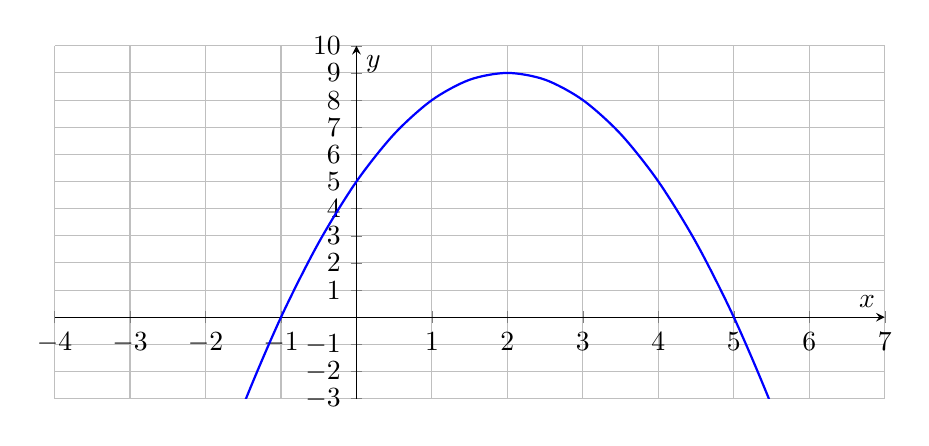
\begin{tikzpicture}
  \begin{axis}[
      xmin = -4.0, xmax = 7.0,
      ymin = -3.0, ymax = 10.0,
      xtick distance = 1.0,
      ytick distance = 1.0,
      major grid style = {lightgray},
      minor grid style = {lightgray!25},
      grid = both,
      width = \textwidth,
      height = 0.5\textwidth,
      axis x line=center,
      axis y line=center,
      xlabel = {$x$},
      ylabel = {$y$},
    ]
      \addplot[
          domain = -4:8,
          smooth,
          thick,
          blue,
      ] {-x^2 + 4*x + 5};
  \end{axis}
  \end{tikzpicture}
  \begin{parts}
    \part
    Geben Sie die Scheitelpunktform der Funktion $f(x)$ an.
    \begin{solution}
      Scheitelpunkt: $S(u,v) = S(2,9)$\\
      $\Rightarrow$ Scheitelpunktform nach Formel $f(x) = a(x-u)^2+v$:
      \[
        f(x) = -(x-2)^2 + 9
      \]
    \end{solution}
    \part
    Bestimmen Sie die Linearfaktordarstellung der Funktion $f(x)$.
    \begin{solution}
      Nullstellen: $x_1 = -1, \quad x_2=5$\\
      $\Rightarrow$ Linearfaktordarstellung nach Formel $f(x) = a(x-x_1)\cdot(x-x_2)$:
      \[
        f(x) = -(x+1)(x-5)
      \]
    \end{solution}
    \part
    Ermitteln Sie die Polynomdarstellung der Funktion $f(x)$.
    \begin{solution}
      Ausmultiplizieren der Scheitelpunktform \textbf{oder} Linearfaktordarstellung liefert:
      \[
        f(x) = -x^2+4x+5
      \]
    \end{solution}
  \end{parts}

  \question
  Gegeben sei die folgende ganzrationale Funktion vierten Grades
  \[
    f(x) = x^4-10x^2+9
  \]
  \begin{parts}
    \part
    Bestimmen Sie alle Nullstellen der Funktion $f(x)$.
    \begin{solution}
      Substitution: $u = x^2$
      \[
        \begin{aligned}
          u^2-10u+9 \\
          u_1 = & \frac{10}{2} + \sqrt{\frac{100}{4} - 9} = 5 + 4 = 9 \\
          u_2 = & 5 - 4 = 1\\
          x_1 = & \sqrt{u_1} = 3 \\
          x_2 = & - \sqrt{u_1} = - 3 \\
          x_3 = & \sqrt{u_2} = 1 \\
          x_4 = & - \sqrt{u_2} = - 1
        \end{aligned}
      \]
    \end{solution}
    \part
    Geben Sie die Gleichung der Funktion $f(x)$ in Linearfaktordarstellung an.
    \begin{solution}
      Mit den Nullstellen $x_1$ bis $x_4$ ergibt sich:
      \[
        f(x) = (x-3)(x+3)(x-1)(x+1)
      \]
    \end{solution}
  \end{parts}

  \question
  Durch Auswertung von Messungen der Ariane 4 Rakete wurde festgestellt, dass sich der Zusammenhang zwischen der Zeit $t$ (in Sekunden) und der Höhe $h$ der Rakete über dem Startplatz (in Metern) bis zum Verlassen der Erdatmosphäre durch eine quadratische Funktion beschreiben lässt. Die folgende Tabelle zeigt die Messwerte:
  \begin{center}
    \begin{tabular}{|l|l|l|l|}
      \hline
      Zeit $t$ in $s$ & $0$ & $20$ & $40$ \\ \hline
      Höhe $h$ in $m$ & $0$ & $760$ & $3040$ \\ \hline
    \end{tabular}
  \end{center}
  Nach welcher Zeit verlässt die Rakete die Erdatmosphäre?
  \begin{solution}
    Funktionsgleichung aufstellen:
    \[
      \begin{aligned}
        760 = a \cdot 20^2 \\
        a = \frac{760}{400} = 1,9
      \end{aligned}
    \]
    $\Rightarrow f(x) = 1,9x^2$\\
    \\
    Erdatmosphäre endet in einer Höhe von $100.000$ m, also diesen Wert in $f(x)$ einsetzen:
    \[
      \begin{aligned}
        100000 = 1,9x^2 \\
        x = \sqrt{\frac{100000}{1,9}} \approx 229,416
      \end{aligned}
    \]
    $\Rightarrow$ Die Rakete verlässt die Erdatmosphäre nach ca. $229,416$ s.
  \end{solution}

  \question
  Innerhalb einer Studie soll die Konzentration eines Medikamentes im Blut untersucht werden. In der Zeitspanne zwischen der Verabreichung des Medikamentes bis zum vollständigen Abbau des Medikamentes wird die Wirkstoffkonzentration im Blut der Probanden (in $\displaystyle \frac{mg}{t}$) durch eine ganzrationale Funktion $f$ beschrieben ($t$ in $h$):
  \[
    f(t) = 0,015t^3-0,6t^2+6t
  \]
  Nach wie vielen Stunden ist kein Wirkstoff mehr im Blut vorhanden?
  \begin{solution}
    Erste Nullstelle durch Ausklammern von $t$:
    \[
      0 = t(0,015t^2-0,6t+6)
    \]
    $\Rightarrow t_1 = 0$ \\
    Weitere Nullstellen durch pq-Formel:
    \[
      \begin{aligned}
        0 = 0,015t^2-0,6t+6 \quad | : 0,015 \\
        0 = t^2-40t+400 \\
        t_2 = 20 + \sqrt{400 - 400} = 20
      \end{aligned}
    \]
    $\Rightarrow$ Nach 20 Stunden ist kein Wirkstoff mehr im Blut.
  \end{solution}

  \question
  Eine Firma produzierte einen besonders umweltfreundlichen PKW in geringer Stückzahl. Die Produktionskosten des Fahrzeugs in Abhängigkeit von der produzierten Stückzahl $x$ werden durch die ganzrationale Funktion $K(x)$ beschrieben: 
  \[
    K(x) = 5x^3-450x^2+16800x+75000
  \]
  Die Fahrzeuge werden zu einem Preis von 20.300 Euro verkauft. Eine erste Hochrechnung ergab, dass bei einem Verkauf von 10 Fahrzeugen die Produktionskosten gedeckt sind.\\
  Ein Unternehmensberater behauptet: ``Mit diesem Gefährt können Sie keinen Gewinn erzielen!''. Beziehen Sie Stellung zu dieser Aussage und begründen Sie Ihre Position.\\
  \textbf{Hinweis:} Der Gewinn ist die Differenz zwischen Erlös und Kosten:
  \[
    G(x) = E(x) - K(x)
  \]
  \begin{solution}
    Ermitteln der Gewinnfunktion $G(x) = -5x^3+450x^2+3500x-75000$.\\
    Nullstelle bei $x_1 = 10$, deshalb Polynomdivision:\\
    \polylongdiv[style=C]{-5x^3+450x^2+3500x-75000}{x-10}\\
    Weitere Nullstelle mit pq-Formel:
    \[
      \begin{aligned}
        0 = -5x^2+400x+7500 \quad | : -5
        0 = x^2-80x-1500 \\
        x_2 = 40 + \sqrt{40^2+1500} = 40 + \sqrt{3100} \approx 95,68 \\
        x_3 = 40 - \sqrt{40^2+1500} = 40 - \sqrt{3100} \approx -15,68
      \end{aligned}
    \]
    $\Rightarrow$ Wenn zwischen 10 und 96 Fahrzeuge verkauft werden, erwirtschaftet das Unternehmen Gewinn. Die Aussage ist also falsch.
  \end{solution}

  \question
  Bei einem Basketballspiel wurde ein Dreipunktewurf analysiert und festgestellt, dass der Ball an seiner höchsten Position eine Höhe von $6,725$ $m$ in einer Entfernung vom Spieler von $3,25$ $m$ erreichen konnte. 
  \begin{parts}
    \part
    Bestimmen Sie die Scheitelpunktform der parabelförmigen Flugbahn des Balls. Die Parabel weist dabei einen Stauchungsfaktor von $\displaystyle \frac{2}{5}$ auf.
    \begin{solution}
      Scheitelpunkt $S(u,v)=S(3,25;6,725)$ in Formel einsetzen:
      \[
        f(x) = -0,4(x-3,25)^2+6,725
      \]
    \end{solution}
    \part
    Ermitteln Sie, in welcher Entfernung der Ball wieder auf dem Spielfeld aufkam.
    \begin{solution}
      Polynomdarstellung bestimmen durch Ausmultiplizieren:
      \[
        f(x) = -0,4x^2+2,6x+2,5
      \]
      Nullstellen bestimmen mit pq-Formel:
      \[
        \begin{aligned}
          0 = -0,4x^2+2,6x+2,5 \quad | : -0,4 \\
          0 = x^2-6,5x-6,25 \\
          x_1 = 3,25 + \sqrt{16,8125} \approx 7,35 \\
          x_2 = 3,25 - \sqrt{16,8125} \approx -0,85
        \end{aligned}
      \]
      $\Rightarrow$ Der Ball kam in einer Entfernung von $7,35$ $m$ auf.
    \end{solution}
    \part
    Geben Sie die Funktionsgleichung in der Linearfaktordarstellung an.
    \begin{solution}
      Mit den Nullstellen $x_1=7,35$ und $x_2=-0,85$ ergibt sich:
      \[
        f(x) = -0,4(x-7,35)(x+0,85)
      \]
    \end{solution}
  \end{parts}

\end{questions}

\end{document}
